\documentclass[12pt, a4, epsf,colorlinks]{amsart}
\usepackage{epsf, amsmath, amssymb, graphicx, epsfig, hyperref, amsthm, mathtools}
\usepackage[utf8]{inputenc}
\usepackage{pgf,tikz,pgfplots}
\usetikzlibrary{arrows}
\usepackage{color}
\usepackage{xcolor}

\begin{document}

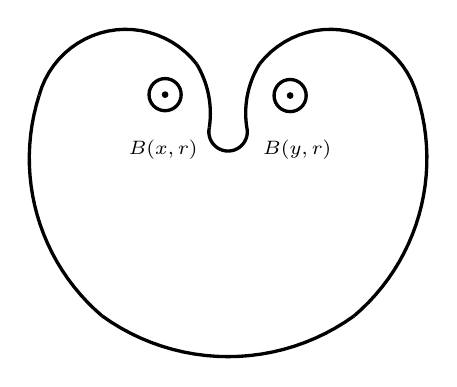
\begin{tikzpicture}[scale=2]
			\draw [shift={(-11.95,8.4)},line width=1.2pt]  plot[domain=2.831889709047336:4.007894916142469,variable=\t]({1*1.3124404748406695*cos(\t r)+0*1.3124404748406695*sin(\t r)},{0*1.3124404748406695*cos(\t r)+1*1.3124404748406695*sin(\t r)});
			\draw [shift={(-12.05,8.4)},line width=1.2pt]  plot[domain=-0.8663022625526775:0.3097029445424578,variable=\t]({1*1.3124404748406684*cos(\t r)+0*1.3124404748406684*sin(\t r)},{0*1.3124404748406684*cos(\t r)+1*1.3124404748406684*sin(\t r)});
			\draw [shift={(-12.65,8.65)},line width=1.2pt]  plot[domain=0.6610431688506853:2.8753406044388665,variable=\t]({1*0.570087712549568*cos(\t r)+0*0.570087712549568*sin(\t r)},{0*0.570087712549568*cos(\t r)+1*0.570087712549568*sin(\t r)});
			\draw [shift={(-11.35,8.65)},line width=1.2pt]  plot[domain=0.2662520491509295:2.4805494847391056,variable=\t]({1*0.5700877125495686*cos(\t r)+0*0.5700877125495686*sin(\t r)},{0*0.5700877125495686*cos(\t r)+1*0.5700877125495686*sin(\t r)});
			\draw [shift={(-12.721132168535297,8.68577126967102)},line width=1.2pt]  plot[domain=-0.14821767022916887:0.5426028080631197,variable=\t]({1*0.6085379462666762*cos(\t r)+0*0.6085379462666762*sin(\t r)},{0*0.6085379462666762*cos(\t r)+1*0.6085379462666762*sin(\t r)});
			\draw [shift={(-11.291769672302514,8.687848474210886)},line width=1.2pt]  plot[domain=2.590802412473704:3.2892961130490246,variable=\t]({1*0.5964366194692994*cos(\t r)+0*0.5964366194692994*sin(\t r)},{0*0.5964366194692994*cos(\t r)+1*0.5964366194692994*sin(\t r)});
			\draw [shift={(-12,8.508196964730805)},line width=1.2pt]  plot[domain=4.087120120443383:5.337657840325996,variable=\t]({1*1.3667847352961513*cos(\t r)+0*1.3667847352961513*sin(\t r)},{0*1.3667847352961513*cos(\t r)+1*1.3667847352961513*sin(\t r)});
			\draw [line width=1.2pt] (-12.39996838597594,8.805243425377359) circle (0.102cm);
			\draw [line width=1.2pt] (-11.606001370593122,8.799405432617192) circle (0.102cm);
			\draw [shift={(-12.000002626550868,8.569245996038335)},line width=1.2pt]  plot[domain=-3.3653023323877065:0.25493143478218927,variable=\t]({1*0.12224130597605011*cos(\t r)+0*0.12224130597605011*sin(\t r)},{0*0.12224130597605011*cos(\t r)+1*0.12224130597605011*sin(\t r)});
			\begin{scriptsize}
			\draw [fill=black] (-12.39996838597594,8.805243425377359) circle (0.5pt);
			\draw[color=black] (-12.412209534460503,8.45619913218483) node {$B(x, r)$};
			\draw [fill=black] (-11.606001370593122,8.799405432617192) circle (0.5pt);
			\draw[color=black] (-11.560739392977234,8.453300886075097) node {$B(y, r)$};
			\end{scriptsize}
			\end{tikzpicture}

\end{document}